\documentclass{article}

% if you need to pass options to natbib, use, e.g.:
% \PassOptionsToPackage{numbers, compress}{natbib}
% before loading nips_2017
%
% to avoid loading the natbib package, add option nonatbib:
% \usepackage[nonatbib]{nips_2017}

\usepackage[final]{nips_2017}

% to compile a camera-ready version, add the [final] option, e.g.:
% \usepackage[final]{nips_2017}

\usepackage[utf8]{inputenc} % allow utf-8 input
\usepackage[T1]{fontenc}    % use 8-bit T1 fonts
\usepackage{hyperref}       % hyperlinks
\usepackage{url}            % simple URL typesetting
\usepackage{booktabs}       % professional-quality tables
\usepackage{amsfonts}       % blackboard math symbols
\usepackage{nicefrac}       % compact symbols for 1/2, etc.
\usepackage{microtype}      % microtypography
\usepackage{float}
\usepackage{graphicx}
\usepackage{changepage}

\title{Wybrane zagadnienia sztucznej inteligencji - Sprawozdanie 3 - Uczenie ze wzmocnieniem i nadzorowane w grach}

% The \author macro works with any number of authors. There are two
% commands used to separate the names and addresses of multiple
% authors: \And and \AND.
%
% Using \And between authors leaves it to LaTeX to determine where to
% break the lines. Using \AND forces a line break at that point. So,
% if LaTeX puts 3 of 4 authors names on the first line, and the last
% on the second line, try using \AND instead of \And before the third
% author name.

\author{Tomasz Pastusiak \And{Leszek Kawecki}}

\begin{document}
% \nipsfinalcopy is no longer used

\maketitle


\section{Badanie Q-learningu}

\subsection{Q-player vs Random}

\begin{figure}[H]
  \centering
  \fbox{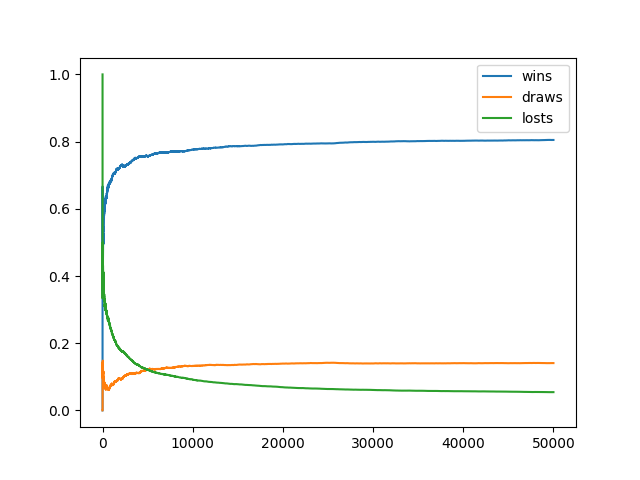
\includegraphics[width=0.9\textwidth]{img/L02G01q_player.png}}
  \caption{Skuteczność w trakcie uczenia}
  \label{fig:L02G01_qlearning}
\end{figure}

\begin{center}
  \begin{tabular}{|l|l|l|l|}
    \hline
    Parametry & wygrana & remis & przegrana \\ \hline
    $\alpha = 0.1, \gamma = 0.1$ & 803 & 155 & 42 \\ \hline
    $\alpha = 0.2, \gamma = 0.1$ & 816 & 146 & 36 \\ \hline
    $\alpha = 0.3, \gamma = 0.1$ & 805 & 147 & 48 \\ \hline
    $\alpha = 0.4, \gamma = 0.1$ & 791 & 147 & 62 \\ \hline
    $\alpha = 0.5, \gamma = 0.1$ & 818 & 129 & 53 \\ \hline
    $\alpha = 0.6, \gamma = 0.1$ & 780 & 170 & 50 \\ \hline
    $\alpha = 0.7, \gamma = 0.1$ & 810 & 141 & 49 \\ \hline
    $\alpha = 0.8, \gamma = 0.1$ & 800 & 140 & 60 \\ \hline
    $\alpha = 0.9, \gamma = 0.1$ & 806 & 143 & 51 \\ \hline
    $\alpha = 1.0, \gamma = 0.1$ & 747 & 154 & 99 \\ \hline
    $\alpha = 2.0, \gamma = 0.1$ & 714 & 152 & 134 \\ \hline\hline
    $\alpha = 0.5, \gamma = 0.2$ & 815 & 124 & 61 \\ \hline
    $\alpha = 0.5, \gamma = 0.3$ & 806 & 145 & 49 \\ \hline
    $\alpha = 0.5, \gamma = 0.4$ & 822 & 133 & 45 \\ \hline
    $\alpha = 0.5, \gamma = 0.5$ & 792 & 161 & 47 \\ \hline
    $\alpha = 0.5, \gamma = 0.6$ & 821 & 137 & 42 \\ \hline
    $\alpha = 0.5, \gamma = 0.7$ & 793 & 153 & 54 \\ \hline
    $\alpha = 0.5, \gamma = 0.8$ & 805 & 130 & 65 \\ \hline
    $\alpha = 0.5, \gamma = 0.9$ & 807 & 130 & 63 \\ \hline
    $\alpha = 0.5, \gamma = 1.0$ & 767 & 167 & 66 \\ \hline
    $\alpha = 0.5, \gamma = 2.0$ & 769 & 126 & 105 \\ \hline
  \end{tabular}
\end{center}

\subsection{Q-player vs Q-Player}

\begin{figure}[H]
  \centering
  \fbox{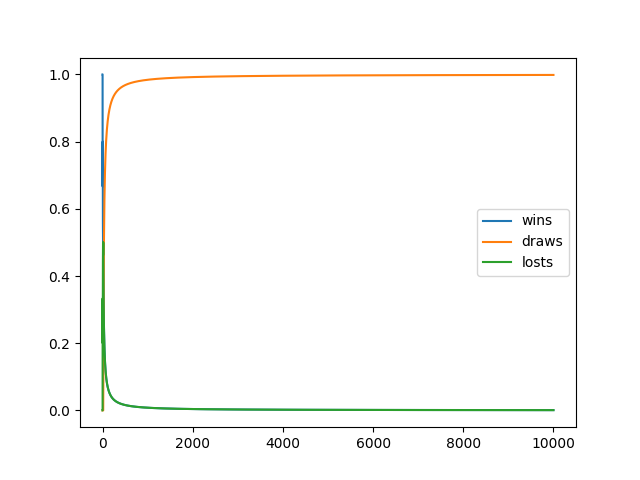
\includegraphics[width=0.9\textwidth]{img/q_player_vs_q_player.png}}
  \caption{Q-player vs Q-player}
  \label{fig:q_player_vs_q_player}
\end{figure}

\section{Badanie uczenia nadzorowanego}

\subsection{Badanie dla sieci neuronowej}

\subsubsection{Wpływ rozmiaru zbioru uczącego na wyniki}

\begin{center}
  \begin{tabular}{|l|l|l|l|}
    \hline
    liczba gier w zbiorze & próba 1 & próba 2 & próba 3 \\ \hline
    2 & (W:450, D:133, L:417) & (W:415, D:148, L:437) & (W:454, D:134, L:412) \\ \hline
    10 & (W:438, D:129, L:433) & (W:483, D:168, L:349) & (W:450, D:107, L:443) \\ \hline
    100 & (W:653, D:58, L:289) & (W:495, D:125, L:380) & (W:442, D:183, L:375) \\ \hline
    500 & (W:652, D:134, L:214) & (W:753, D:118, L:129) & (W:718, D:76, L:206) \\ \hline
    1000 & (W:676, D:178, L:146) & (W:431, D:154, L:415) & (W:841, D:78, L:81) \\ \hline
    5000 & (W:869, D:86, L:45) & (W:848, D:114, L:38) & (W:913, D:54, L:33) \\ \hline
    10000 & (W:914, D:50, L:36) & (W:865, D:110, L:25) & (W:907, D:55, L:38) \\ \hline
  \end{tabular}
\end{center}

\subsubsection{Wpływ graczy użytych do generowania zbioru uczącego}

\begin{center}
  \begin{tabular}{ | l | l | l | l | }
    \hline
    użyci gracze & próba 1 & próba 2 & próba 3 \\ \hline
    RandomPlayer vs RandomPlayer & (W:801, D:100, L:99) & (W:746, D:181, L:73) & (W:469, D:133, L:398) \\ \hline
    MLPPlayer vs RandomPlayer & (W:441, D:132, L:427) & (W:375, D:85, L:540) & (W:439, D:154, L:407) \\ \hline
    MLPPlayer vs MLPPlayer & (W:498, D:131, L:371) & (W:516, D:123, L:361) & (W:415, D:159, L:426) \\ \hline
    RandomPlayer vs RandomPlayer & (W:747, D:163, L:90) & (W:793, D:84, L:123) & (W:825, D:80, L:95) \\ \hline
  \end{tabular}
\end{center}

\subsection{Badanie dla drzewa decyzyjnego}

\subsubsection{Wpływ rozmiaru zbioru uczącego na wyniki}

\begin{center}
  \begin{tabular}{ | l | l | l | l | }
    \hline
    liczba gier w zbiorze & próba 1 & próba 2 & próba 3 \\ \hline
    2 & (W:530, D:140, L:330) & (W:455, D:124, L:421) & (W:399, D:147, L:454) \\ \hline
    10 & (W:398, D:105, L:497) & (W:462, D:129, L:409) & (W:485, D:109, L:406) \\ \hline
    100 & (W:587, D:67, L:346) & (W:552, D:120, L:328) & (W:523, D:104, L:373) \\ \hline
    500 & (W:577, D:125, L:298) & (W:622, D:90, L:288) & (W:615, D:65, L:320) \\ \hline
    1000 & (W:661, D:87, L:252) & (W:659, D:91, L:250) & (W:637, D:93, L:270) \\ \hline
    5000 & (W:794, D:90, L:116) & (W:825, D:49, L:126) & (W:804, D:74, L:122) \\ \hline
    10000 & (W:876, D:39, L:85) & (W:887, D:62, L:51) & (W:899, D:67, L:34) \\ \hline
  \end{tabular}
\end{center}

\subsubsection{Wpływ graczy użytych do generowania zbioru uczącego}

\begin{center}
  \begin{tabular}{ | l | l | l | l | }
    \hline
    użyci gracze & próba 1 & próba 2 & próba 3 \\ \hline
    RandomPlayer vs RandomPlayer & (W:666, D:92, L:242) & (W:681, D:57, L:262) & (W:686, D:92, L:222) \\ \hline
    MLPPlayer vs RandomPlayer & (W:572, D:99, L:329) & (W:483, D:118, L:399) & (W:463, D:137, L:400) \\ \hline
    MLPPlayer vs MLPPlayer & (W:499, D:129, L:372) & (W:503, D:115, L:382) & (W:474, D:70, L:456) \\ \hline
    RandomPlayer vs RandomPlayer & (W:646, D:86, L:268) & (W:654, D:66, L:280) & (W:695, D:95, L:210) \\ \hline
  \end{tabular}
\end{center}

\subsection{Bratobójcze walki}

Dla zbioru uczącego zawierającego 1000 gier

\begin{center}
  \begin{tabular}{ | l | l | l | l | }
    \hline
    użyci gracze & próba 1 & próba 2 & próba 3 \\ \hline
    Tree vs Tree & (W:449, D:30, L:521) & (W:443, D:78, L:479) & (W:538, D:60, L:402) \\ \hline
    MLP vs MLP & (W:795, D:118, L:87) & (W:115, D:157, L:728) & (W:500, D:0, L:500) \\ \hline
    MLP vs Tree & (W:299, D:109, L:592) & (W:212, D:73, L:715) & (W:317, D:90, L:593) \\ \hline
  \end{tabular}
\end{center}


\section{Porównanie Q-learningu i uczenia nadzorowanego}



\end{document}
